\documentclass[usenames, dvipsnames, aspectratio=32]{beamer}
\usepackage[utf8]{inputenc}
\usepackage[T1]{fontenc}
\usepackage[english]{babel}
\usepackage[defaultfam, regular]{montserrat}
\usepackage{csquotes}
\usepackage[normalem]{ulem}
\usepackage{latexsym,multicol,booktabs,miama}
\usepackage{setspace}
\usepackage{xcolor}
\usepackage{pgfplots,pgfpages}
\usepackage{tikz}
    \usetikzlibrary{calc}
\usepackage{amssymb,amsfonts,amsmath,amsthm,mathrsfs,mathptmx} 
\usepackage{graphicx,pstricks,listings,stackengine,multirow}
\usepackage{adjustbox}
\usepackage[backend=biber,bibencoding=utf8,urldateusetime=true,style=alphabetic,sorting=nyt,natbib=true]{biblatex}
\usepackage{style}
\usepackage{hyperref}
    \hypersetup{colorlinks=true, citecolor=BrickRed, filecolor=black, linkcolor=main, urlcolor=blue}

% \setbeamertemplate{note page}[plain]
% \setbeameroption{show notes on second screen=right}
% \setbeamertemplate{note page}{\pagecolor{yellow!5}\vfill\insertnote\vfill}

\makeatletter
\def\beamer@setupnote{%
  \gdef\beamer@notesactions{%
    \beamer@outsideframenote{%
      \beamer@atbeginnote%
      \beamer@notes%
      \ifx\beamer@noteitems\@empty\else
      \begin{itemize}%
        \setlength{\itemsep}{.4em}
        \setlength{\topsep}{.3em}
        \setlength{\parsep}{0pt}
        \beamer@noteitems%
      \end{itemize}%
      \fi%
      \beamer@atendnote%
    }%
    \gdef\beamer@notesactions{}%
  }
}
\makeatother

\setbeamertemplate{bibliography item}{\insertbiblabel}
\setbeamertemplate{caption}[numbered]
\addbibresource{../report/refs.bib}


\author[Malte Grube]{\vspace*{-.8em}Malte Grube\inst{1}}
\title[]{Surprise Adequacy (SA)}
\subtitle{--\; SE4AI Präsentation \;--}
\institute[Uni Rostock]{
    \inst{1}
    \footnotesize{Dozentin: \textit{Prof. Dr. rer. nat. Regina Hebig}} \vspace{.25em} \\
    Universität Rostock
}
\date{01. Juli 2026}

\def\cmd#1{\texttt{\color[RGB]{0, 0, 139}\footnotesize $\backslash$#1}}
\def\env#1{\texttt{\color[RGB]{0, 0, 139}\footnotesize #1}}

\lstdefinestyle{texstyle}{
    language=[LaTeX]TeX,
    basicstyle=\ttfamily\footnotesize,
    keywordstyle={\bfseries\color[RGB]{0, 0, 180}},
    keywordstyle=[2]{\slshape\color[RGB]{225, 140, 30}},
    morekeywords=[2]{,itemize, enumerate, equation, table, tabular},
    stringstyle=\color[RGB]{50, 50, 50},
    numbers=left,
    numberstyle=\footnotesize\color{gray},
    rulesepcolor=\color{red!20!green!20!blue!20},
    frame=shadowbox
}

\AtBeginBibliography{\scriptsize}

\begin{document}
{
\setbeamertemplate{headline}{}
\begin{frame}
    \vspace*{1em}
    \begin{figure}[htpb]
    \centering
    
\includegraphics[width=0.55\linewidth]{logo.jpg}
    \end{figure}
    \vspace*{-1.5em}
    \titlepage
\end{frame}
}

\begin{frame}
    \tableofcontents[sectionstyle=show,subsectionstyle=show/shaded/hide,subsubsectionstyle=show/shaded/hide]
    % \note{\begin{itemize}
    %     \setlength{\itemsep}{1em}
    %     \item 
    %     \item 
    % \end{itemize}}
\end{frame}

\section{Besonderheit von SA}

\begin{frame}{Motivation}
    \begin{itemize}
        \item \textbf{Softwareentwicklung}: Bewertung der Qualität von \textit{Testfällen} (Statement-Coverage, Branch-Coverage, ...) % wie viel % der ausführbaren Codezeilen werden von Testfällen mindestens einmal durchlaufen? / bzw wie viele verzweigungen
        \item \textbf{Neuronale Netze}: Keine Kontrollflussstrukturen \\$\to$ Metriken \textit{nicht anwendbar} \cite{sa_1,sa_2}
    \end{itemize}
\end{frame}

\begin{frame}{Metrik für neuronale Netze}
    \begin{itemize}
        \item \textbf{Neuron Coverage (NC)} \cite{neuron_coverage}: Wie viele Neuronen- Aktivierungen überschreiten \textit{Schwellenwert} im Netz?
        \item \textbf{Problem}: \textit{Kontinuierliche} Werte der Neuronen nicht ausreichend berücksichtigt \cite{sa_1,sa_2} % da man dies auf eine Binärentscheidung reduziert 
    \end{itemize}
\end{frame}

\begin{frame}{Autoren von Surprise Adequacy (SA)}
    \begin{itemize}
        \item \textbf{Kim et al.}\,\cite{sa_1,sa_2}: Messung der ''Überraschung'' einer \textit{neuen Eingabe}
        \item In Relation zu den Trainingsdaten % um unerwartetes Modellverhalten identifizieren zu können
    \end{itemize}
\end{frame}

\begin{frame}{Activation Traces (ATs)}
    \begin{itemize}
        \item \textbf{Aktivierungen} der Neuronen einer Schicht im Netz
        \item Vektor als Muster für \textit{jeweiliges} Input-Bild analysiert
    \end{itemize}
\end{frame}

\begin{frame}{Ziel von SA}
    \begin{itemize}
        \item \textbf{Quantifizierung} der Vielfältigkeit einer Test-Suite
        \item Auch mit \textit{manipulierten} Bildern möglich % in sicherheitskritischen Anwendungen (autonomes Fahren, medizinische Bildgebung) braucht man vor allem Test-Cases, um Korrektheit und Robustheit zu prüfen
    \end{itemize}
\end{frame}

\begin{frame}{Ziel von SA}
    \begin{figure}
        \centering
        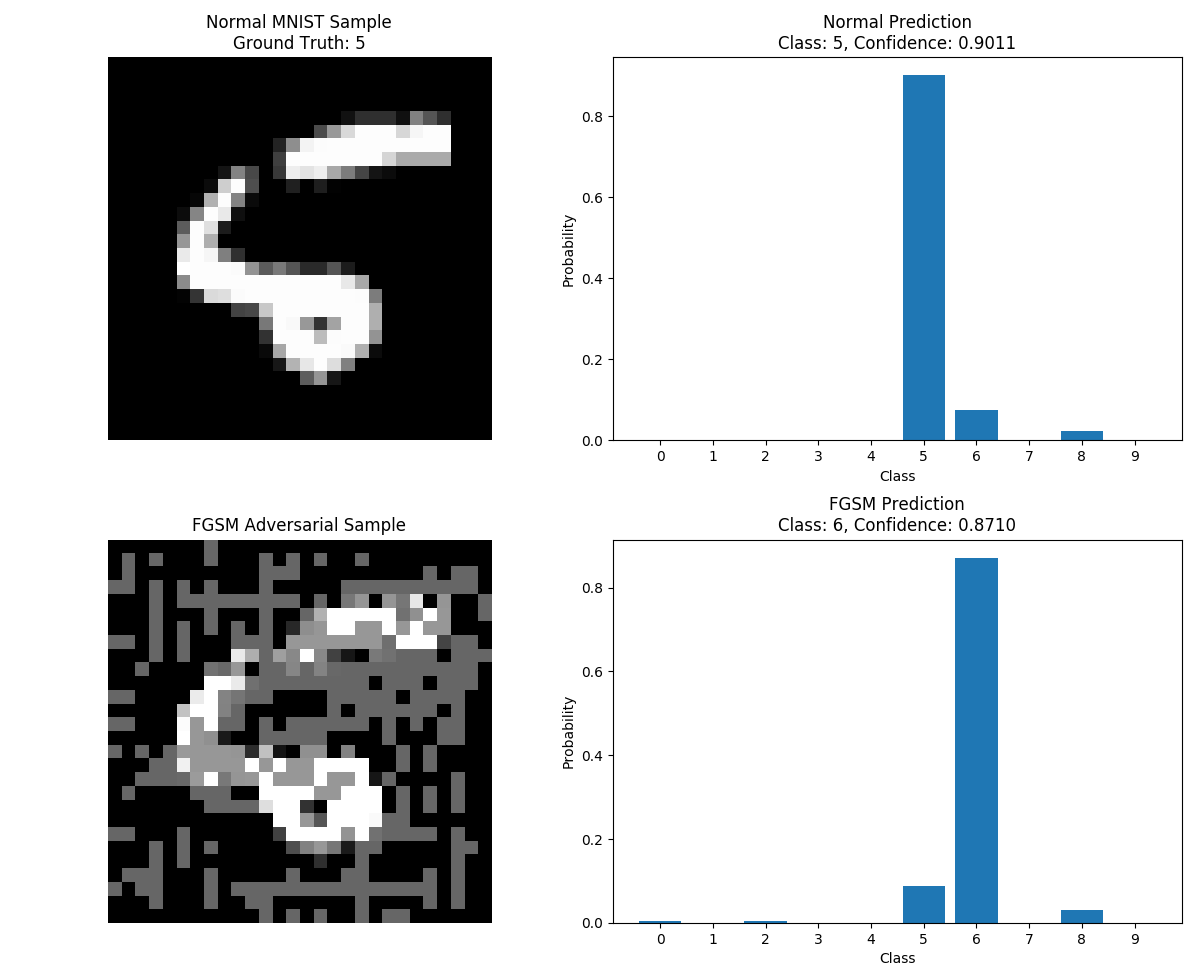
\includegraphics[width=0.5\linewidth]{../report/img/prediction_5.png}
        \caption{Vorhersage einer ''5''. Das Test-Bild wurde mit hoher Wahrscheinlichkeit korrekt klassifiziert, während das FGSM-Bild stattdessen als ''6'' klassifiziert wurde.}
    \end{figure}
\end{frame}

\section{Funktionsweise von SA}

\begin{frame}{Grundlegendes Prinzip}
    \begin{enumerate}
        \item Für jedes \textbf{Trainingsbeispiel}: Berechnung der ATs
        \item Für jedes \textbf{Testbeispiel}: Berechnung der ATs
        \item \textbf{SA}-Verfahren anwenden (LSA, DSA, MDSA)
        \item \textbf{Ergebnis}: SA-Wert für jedes Testbeispiel
        \item \textbf{Surprise Coverage (SC)}: Bewertung der Test-Suite
    \end{enumerate}
\end{frame}

\begin{frame}{Likelihood-based SA (LSA)}
    \begin{enumerate}
        \item \textbf{Train-ATs}: Kernel Density Estimation (KDE)
        \item \textbf{Test-AT}: Berechnung der Dichte für $x$
        \item \textit{Niedrige Dichte $\to$ höhere Überraschung} % ungewöhnlicher AT bzgl. Train-AT-Verteilung
    \end{enumerate}
        \vspace{1em}
        $$LSA(x) = -\log(\hat{f}(x))$$
\end{frame}

\begin{frame}{Distance-based SA (DSA)}
    \begin{enumerate}
        \item Berechnung 2 \textbf{Euklidischer Distanzen}: % alle Train-ATs sind bestimmt worden, und im AT-Raum zu finden 
        \begin{enumerate}
            \item $dist_a$: Test-AT $\to$ nächster Train-AT \textit{derselben} Klasse \vspace{.3em}
            \item $dist_b$: Train-AT $\to$ nächsten Train-AT \textit{anderer} Klasse \vspace{.2em}
        \end{enumerate}
        \item Für \textbf{Test-AT} $x$: 
    \end{enumerate}
    $$DSA(x) = \frac{dist_a}{dist_b}$$ \vspace{-.2em}
    \begin{itemize}
        \item Kleiner Abstand zu \textbf{gleicher} Klasse $\to$ kleine DSA % vor allem nah an der Entscheidungsgrenze ist DSA hoch
    \end{itemize}
\end{frame}

\begin{frame}{Mahalanobis Distance-based SA (MDSA)}
    \begin{enumerate}
        \item Für \textbf{Train-ATs}:
        \begin{enumerate}
            \item Berechnung des Mittelwertsvektors $\mu$ (einmalig) \vspace{.3em}
            \item Berechnung der Kovarianzmatrix $C$ (einmalig) \vspace{.2em}
        \end{enumerate}
        \item Für \textbf{Test-AT} $x$:
    \end{enumerate}
    $$MDSA(x) = \sqrt{(x - \mu)^T C (x - \mu)}$$ \vspace{-.2em} % Streuungen und Abhängigkeiten der ATs berücksichtigt (Form der Verteilung der Train-ATs)
    \begin{itemize}
        \item Test-AT \textbf{nah am Zentrum} $\to$ niedrige MDSA % während weit entfernte Test-ATs unbekannte oder manipulierte Daten repräsentieren könnten
        \item Industrieller Einsatz durch \textbf{Effizienz} möglich % da Vergleiche mit Train-ATs nicht notwendig, kann man auf großen Modellen und Datensätzen wie ImageNet anwenden
    \end{itemize}
\end{frame}

\begin{frame}{Surprise Coverage (SC)}
    \begin{itemize}
        \item \textit{Reminder zu NC}: \#Neuronenakt. über Schwellenwert % stieg mit schrittweisem Hinzufügen von adversarialen Testfällen kaum an
        \item SC prüft \textbf{Vielfältigkeit} der Test-Suite via SA-Verteilung:\vspace{.3em}
        \begin{enumerate}
            \item $n$ Buckets für SA-Werte definieren \textcolor{gray}{(z.B.\, $n=1000$)} \vspace{.3em}
            \item LSA-Werte der \textbf{Testbeispiele} in Buckets einordnen \vspace{.6em} % in wie vielen dieser Buckets gibt es mindestens ein Testbeispiel?
            \item SC = $\displaystyle\frac{\#\text{Buckets mit } \geq 1\text{ Testbeispielen}}{n}$ \vspace{.5em}
            \item \textbf{Ergebnis}: Coverage-Wert zwischen $[0,1]$
        \end{enumerate} 
    \end{itemize}
\end{frame}

\section{Hands-on Beispiel}

\begin{frame}{Hands-on: DSA mit MNIST}
    \begin{itemize}
        \item \textbf{Annahme}: ATs liegen in 2D-Raum vor
        \item \textbf{Euklidischer Distanz} $\to$ DSA-Werte berechnen
        \item \textbf{Vier Punkte} im Raum (2x Test, 2x Train) \vspace{.3em}
        \begin{enumerate}
            \item Test-AT für Klasse ''5'': $(3,2)$ \vspace{.3em}
            \item Manipulierter Test-AT für Klasse ''5'': $(10,8)$ \vspace{.3em}
            \item Train-AT für Klasse ''5'': $(2,2)$ \vspace{.3em}
            \item Train-AT für Klasse ''6'': $(6,2)$ \vspace{.3em}
        \end{enumerate}
    \end{itemize}
\end{frame}

\section{Repository-Erfahrungen}

\begin{frame}[allowframebreaks]{Repository-Erfahrungen}
    \begin{itemize}
        \item LSA mit MNIST lokal berechnet
        \item Test-Set und FGSM-Set analysiert % jeweils 10.000 Bilder
        \item Es folgen nun Plots...
    \end{itemize}
    \framebreak
    \begin{figure}
        \centering
        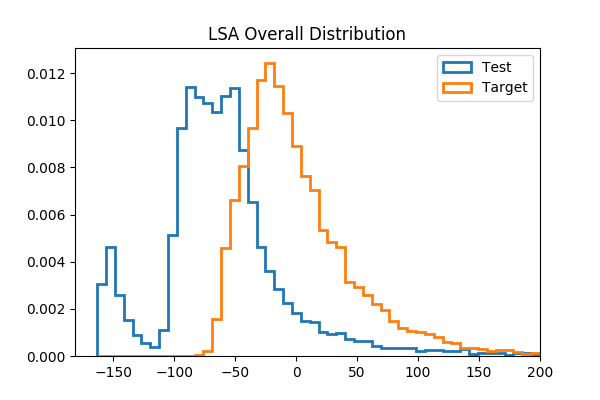
\includegraphics[width=0.6\linewidth]{../report/img/lsa_overall.png}
        \caption{Akkumulierte LSA-Verteilungen für das MNIST-Testset zwischen Original- und FGSM-Bildern.}
    \end{figure}
    \framebreak
    \begin{figure}
        \centering
        \begin{minipage}{0.48\textwidth}
            \centering
            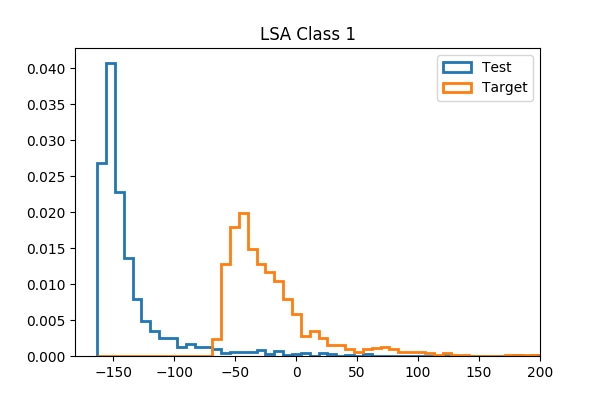
\includegraphics[width=\linewidth]{../report/img/lsa_class_1.png}
            \caption{LSA-Verteilungen für die Klasse ''1''.}
        \end{minipage}\hfill
        \begin{minipage}{0.48\textwidth}
            \centering
            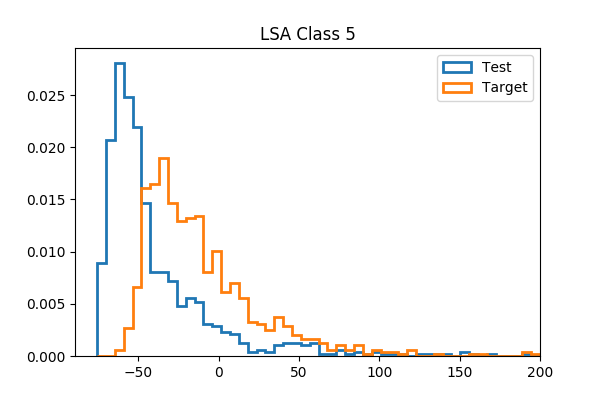
\includegraphics[width=\linewidth]{../report/img/lsa_class_5.png}
            \caption{LSA-Verteilungen für die Klasse ''5''.}
        \end{minipage}
    \end{figure} % FGSM zeigt grundsätzlichen Rechtsdrift in Verteilung, höhere LSA-Werte an sich
    \framebreak
    \begin{itemize}
        \item \textbf{Weitere} Adversarial-Datensätze einbauen, um schritt- weise die Surprise Coverage zu erhöhen \cite{sa_1,sa_2}
        \item Im Nachfolgepaper \cite{sa_2}:
        \begin{itemize}
            \item \textbf{LSC}: 34.1\% auf 71\% \vspace{.3em}
            \item \textbf{DSC}: 46\% auf 74.2\% \vspace{.3em}
            \item \textbf{MDSC}: 54.5\% auf 82.2\%
        \end{itemize}
    \end{itemize}
    % das klingt vielversprechend, aber die Implementierung ist sehr alt (Python 3.5, Tensorflow 1.9), und vieles aus den Veröffentlichungen ist nicht ausprobierbar/reproduzierbar
    % z.B. kein Seeding overall, Mischung von Datensätzen für SC-Verbesserung nicht möglich, Ergebnisse letztendlich stark vom Modell und den gelernten Parametern selbst abhängig
\end{frame}

\section{Fazit}

\begin{frame}[allowframebreaks]{Fazit}
    \begin{itemize}
        \item \textbf{SA}: Vielfalt von Test-Suites für NN quantifizieren
        \item \textbf{LSA, DSA, MDSA}: verschiedene Ansätze % zur Berechnung
        \item \textbf{SC}: Bewertung der Test-Suite basierend auf SA-Vielfalt
        % Bilder wie FGSM sollen System zu falschen Vorhersagen zwingen, um unerwartetes Fehlverhalten/Probleme in der echten Welt zu repräsentieren
    \end{itemize}
    \framebreak
    \begin{itemize}
        \item Auswahl von Testfällen \textbf{über SA-Spektrum} hinweg sinnvoll für Retraining \cite{sa_1}
        \item \textbf{Gewinn gering} in umfassenden Experimenten \cite{sa_2} % ein überraschendes Bild gibt keine Garantie für Modellverbesserung
        \item Im Gegensatz zu XAI kann SA \textbf{nicht angeben}, warum Modell Vorhersage getroffen hat
    \end{itemize}
\end{frame}

\appendix
\setbeamertemplate{headline}{}
\begin{frame}{References}
    \printbibliography[heading=none]
\end{frame}

\begin{frame}
    \centering
    \vspace{1em}
    \huge \textcolor{Black!80}{Vielen Dank fürs Zuhören!}
\end{frame}

\end{document}
